\chapter{ミリ波観測法}
\label{ch:mm_obs}
\ref{ch:mm_obs}章では、我々が開発したミリ波分光計を用いた大気分子の観測手法について述べる。
まず\ref{sec:mm_obs}節では観測手法の概観を紹介し、観測された電波強度のキャリブレーション方法、受信電波から分子スペクトルを抽出するために行う周波数スイッチング、下層大気の影響を評価し除去するための光学的厚みの測定について述べる。
次に、本研究で使用したミリ波分光計について、\ref{subsec:mm_tromsoe}節でノルウェーのトロムソに設置した装置、\ref{subsec:mm_syowa}節で南極の昭和基地に設置された装置についてそれぞれ説明する。


\section{観測手法}
\label{sec:mm_obs}
\subsection{観測手法の概観と観測装置}
最初に、ミリ波分光法を用いた大気分子の観測手法について述べる。
私たちのグループでは、観測の手法としてミリ波電波分光法による地上観測によって大気分子を観測している~\cite{mizuno2002millimeter}。
その模式図を図\ref{fig:spectrometer_schema}に示す。
\begin{figure}[htbp]
    \centering
    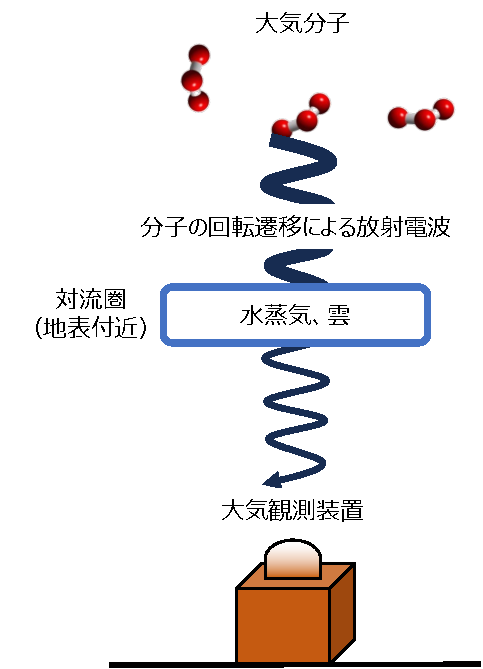
\includegraphics{master_thesis_contents/master_thesis_fig/spectrometer_schema.pdf}
    \caption{ミリ波電波分光法による地上観測の模式図}
    \label{fig:spectrometer_schema}
\end{figure}
% 「下層大気」
% この場合、「下層大気」とは何でしょうか?高度軸は、対流圏・成層圏などの言葉を使い(もしくは高度を数字で書いても良い)、もう少し正確・定量的に描いた方が良い。
ミリ波電波分光法では、観測対象の大気分子の回転遷移によって放射されるミリ波帯電波を受信し分光することで、電波放射スペクトルを観測している。
しかし、図\ref{fig:spectrometer_schema}に示す通り、電波を地上で観測すると、経路上にある下層大気の水蒸気や雲の影響を考慮する必要があることに注意しなければならない。
この影響は、下層大気の光学的厚みを実際に計測することで、補正ができる。
光学的厚みの測定方法の詳細は\ref{subsec:opticaldepth}節にて述べる。\par

ミリ波分光計を用いた大気観測装置の構成を図\ref{fig:mm_component}に示し、例として南極の昭和基地に設置された大気観測装置の様子を図\ref{fig:mmobs_spectrometer_syowa}に示す。
図\ref{fig:mm_component}に示すように、観測装置は主に以下の4つの部分に分かれている。
\begin{figure}[htbp]
    \centering
    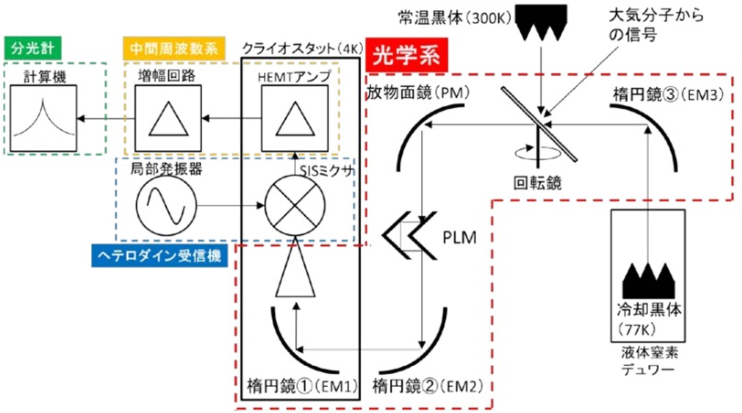
\includegraphics[width=\linewidth]{master_thesis_contents/master_thesis_fig/mm_component.pdf}
    \caption{ミリ波大気観測装置の概略図(~\cite{ito2017master}より引用)}
    % \caption{$\scriptstyle \mbox{ミリ波大気観測装置の概略図}\atop \scriptstyle \mbox{text}(~\cite{ito2017master}より引用$}
    \label{fig:mm_component}
\end{figure}
\begin{figure}[htbp]
    \centering
    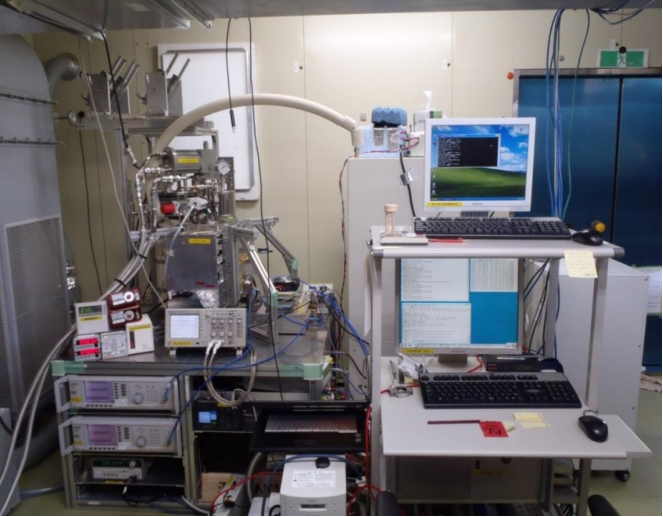
\includegraphics[width=\linewidth]{master_thesis_contents/master_thesis_fig/mmobs_spectrometer_syowa.pdf}
    \caption{南極の昭和基地に設置された観測装置(~\cite{uemura2014master}より引用)}
    \label{fig:mmobs_spectrometer_syowa}
\end{figure}
\begin{enumerate}
    \item 光学系 \par
        大気分子からの信号を集光し伝送するための複数の鏡と電磁ホーンによって構成される。
        また、回転鏡を用いることにより、強度キャリブレーションに用いる基準雑音信号として、常温黒体($300\, \mathrm{K}$)と冷却黒体($77\, \mathrm{K}$)からの放射も入力できるようになっている。
        大気分子からの信号とその信号のキャリブレーション(詳細は\ref{subsec:calibration}節)で用いる常温黒体と冷却黒体の測定との切り替えを行う。
        PLM(光路長変調器: Path Length Modulator)は光学系にて発生する定常波を除去する役割がある。
    \item ヘテロダイン受信機 \par
        大気分子からの信号を局部発振器からの信号とSISミクサで混合する。
        大気分子からの電波は微弱であるため、信号処理に適切なレベルまで増幅しなければならない。
        しかし、本研究で扱う電波の周波数(数百GHz程度)を直接増幅できる増幅器は、現在のところ実用レベルでは存在しない。
        そこで、受信した信号をSISミクサを用いて低い周波数(数GHz程度)に下げることにより、一般的なマイクロ波帯のHEMTアンプによって増幅する方法をとっている。
        このような受信方法をヘテロダイン方式と呼ぶ。
    \item 中間周波数系 \par
        ミクサから出力された信号を後段の分光計にとって適切な周波数にさらに変換し、必要な電波強度レベルまで増幅する。
    \item 分光計 \par
        入力信号を直接A/D変換して時系列データとして読み込み、それを高速フーリエ変換することにより大気分子の周波数スペクトルを得る。
        本研究で用いた大気分子のスペクトルデータを得るために使用された分光計は
        % 追加:「、**社の**であり、その仕様としては」
        16348チャンネルの周波数スペクトルデータを出力する~\cite{ito2017master}。
        % 昭和基地の場合のチャンネル数は?引用元をみないといけない
        % もし分光計の仕様を紹介したいのであれば、チャネル数だけを書くというのはあまり意味がありません。たとえば、大山さんの論文を見て、分光計の諸元として何が書かれているかを参考にすると良い。
\end{enumerate} \par
ミリ波電波分光法による地上観測による最大の利点は、太陽光などの背景光源を必要としないため、昼夜を問わず連続的なモニタリングが可能なことである。
これは、昼夜だけでなく白夜や極夜がある極地においても、その影響を受けずに連続観測することができる唯一の手法であることを意味している。
以上より、連続的・長期的に観測を行うことが可能で、一地点において観測することにより自然起源や人為起源による長期的変動や短期的変動を観測することが可能であり、これが我々の研究グループがミリ波電波分光法による地上観測という世界的に見てもユニークな手法に力を入れている理由である。

\subsection{電波強度のキャリブレーション}
\label{subsec:calibration}
次に、観測された電波に対して黒体を用いて行う強度キャリブレーションの手法について述べる。
一般的に電波領域の研究では、大気分子からの電波放射強度は、それと同等のエネルギーを放射する黒体の温度に換算して表す。ここでミリ波領域(周波数$30-300\, \mathrm{GHz}$)においては、図\ref{fig:planck}よりRayleigh-Jeans近似が成り立つので、ほぼPlanckの放射式は以下のように表すことができる。
\begin{gather}
    I_{\nu}(T)
    = \frac{2\mathrm{h}\nu^3}{c^2} \cdot \cfrac{1}{\exp \Biggl( \cfrac{\mathrm{h}\nu}{\mathrm{k}T}-1\Biggr) }
    \approx \frac{2\mathrm{h}\nu^3}{c^2} \cdot \left(\frac{\mathrm{h}\nu}{\mathrm{k}T}\right)^{-1}
    = \frac{2\nu^2}{c^2}\mathrm{k}T \\
    I_\nu(T):電波強度、c:光速、\mathrm{k}:Boltzmann定数、\mathrm{h}:Planck定数、\nu:周波数、T:黒体温度 \notag
    \label{eq:planck}
\end{gather}
\begin{figure}[htbp]
    \centering
    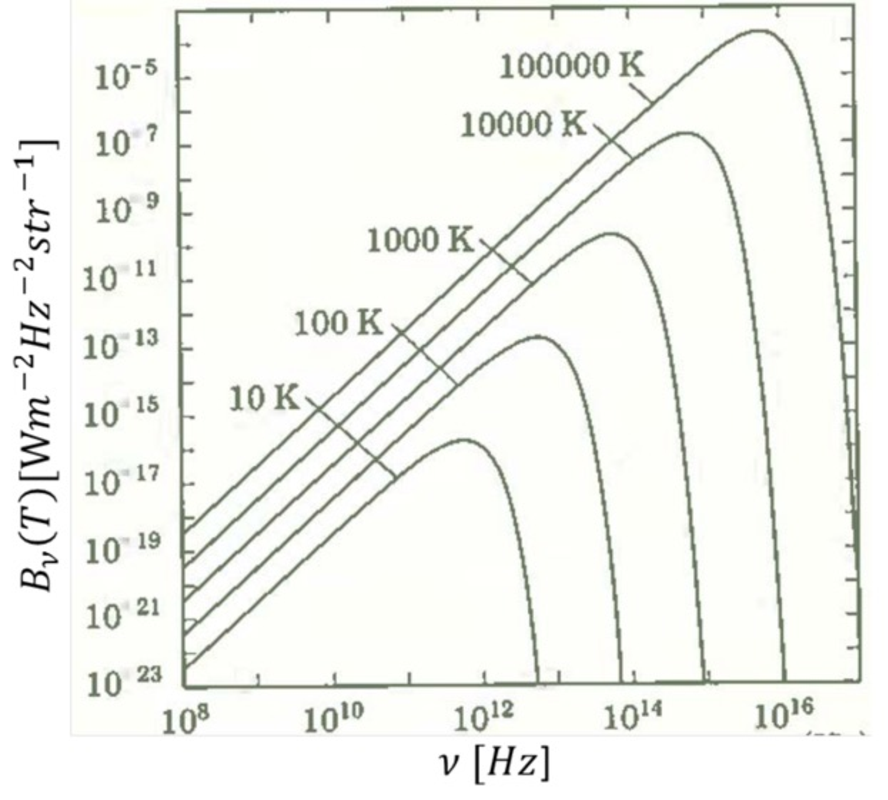
\includegraphics[width=\linewidth]{master_thesis_contents/master_thesis_fig/planck.pdf}
    \caption{Planckの放射式(~\cite{ito2017master}より引用)}
    \label{fig:planck}
\end{figure}
この式から黒体温度と電波強度は比例の関係になるため、大気分子からの電波強度を黒体の温度に換算することが可能である。
具体的には常温黒体(多くの場合室温の$300\ \mathrm{K}$)と液体窒素で冷却された黒体($77\ \mathrm{K}$)からの電波放射を受信機に入れることにより、受信電波強度を黒体の温度スケーリングする(これを強度較正あるいは強度キャリブレーションと呼ぶ)。
\begin{figure}[htbp]
    \centering
    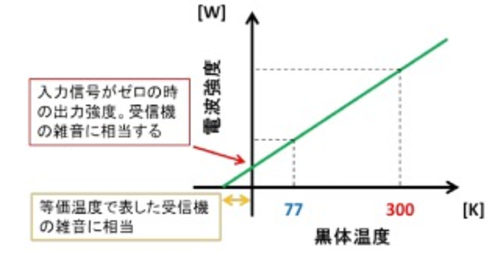
\includegraphics[scale=0.6]{master_thesis_contents/master_thesis_fig/calibration.pdf}
    \caption{電波強度のキャリブレーションの様子(~\cite{ito2017master}より引用)}
    \label{fig:calibration}
\end{figure}
これを図示すると、図\ref{fig:calibration}に示す直線が電波強度と黒体温度の対応を表す。
また、この直線の$y$切片の値は受信機雑音の強度を表し、$x$切片の値の絶対値はこの強度を黒体温度で表した値となる。


\subsection{光学的厚み}
\label{subsec:opticaldepth}
次に、受信された電波強度について、下層大気の影響の補正に用いる光学的厚みについて述べる。
図\ref{fig:spectrometer_schema}に示したように、成層圏よりも高い高度にある分子からの電波を地上で観測する際には、下層大気(主に対流圏)を通過してきた電波を観測することになる。
そのため、下層大気に含まれる水蒸気や雲の放射および吸収の影響を考慮に入れる必要があり、光学的厚みという概念を導入する。\par

まず、光学的厚みとは何かということと、それがどのように電波強度に影響するかを述べる。
図\ref{fig:depth_dx}のように、厚さ$dx$の大気層があり、図の左から強度$T$の電波が入射したときを考える。
大気層で吸収および放射の影響を受けて、図の右に出てくる電波強度は$T+dT$で表される。
\begin{figure}[htbp]
    \centering
    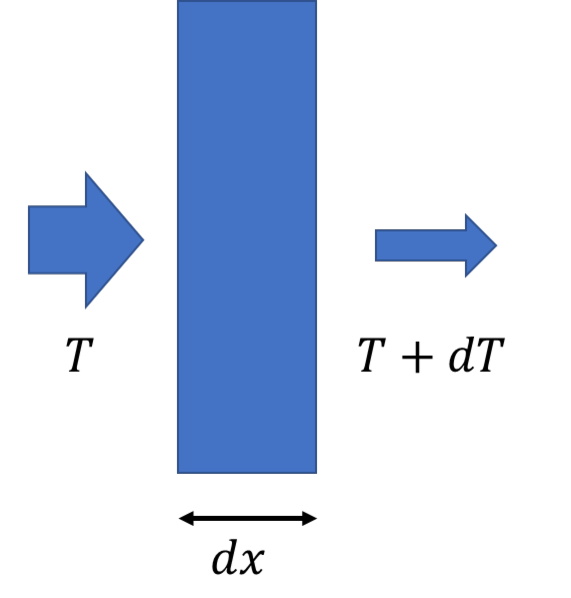
\includegraphics{master_thesis_contents/master_thesis_fig/depth_dx.pdf}
    \caption{厚さ$dx$の大気層を通過する電波強度の模式図}
    \label{fig:depth_dx}
\end{figure}
このとき、吸収と自己放射を表す式は、$\kappa$を吸収係数、$j$を放射係数とすると
\begin{equation}
    dT = -\kappa T dx + j dx
    \label{eq:absorption_selfemission_1}
\end{equation}
となる。
次に光学的厚み(一般的に$\tau$で表す)を導入する。$\tau$は、
\begin{equation}
    \tau = \int_{0}^{x} \kappa dx' + j dx
\end{equation}
もしくは
\begin{equation}
    d\tau = \kappa dx
\end{equation}
と表され、これを用いて式\eqref{eq:absorption_selfemission_1}を書き換えると
\begin{equation}
    \frac{dT}{d\tau} = -T + \frac{j}{\kappa}
    \label{eq:absorption_selfemission_4}
\end{equation}
となる。
次に、式\eqref{eq:absorption_selfemission_4}の第2項において、熱平衡状態ではキルヒホッフの法則より
\begin{gather}
    \frac{j}{\kappa}
    = \frac{2\mathrm{h}\nu^3}{c^2} \cdot \cfrac{1}{\exp\Biggl(\cfrac{\mathrm{h}\nu}{\mathrm{k}T}-1\Biggr)}
    \equiv I_\nu
    = T_\mathrm{sky}
    \label{eq:absorption_selfemission_5} \\
    % I_\nu :電波強度、T_{sky}:大気からの熱放射、c:光速、k:Boltzmann定数 \notag \\
    % h:Planck定数、\nu :周波数、T:黒体温度 \notag
    T_\mathrm{sky}:大気からの熱放射 \notag
\end{gather}
が成り立つ。
これを利用して式\eqref{eq:absorption_selfemission_5}より式\eqref{eq:absorption_selfemission_4}の解を求めると、
\begin{gather}
    T = T_0\exp\left(-\tau\right) + T_\mathrm{sky}\left(1-\exp\left(-\tau\right)\right) + T_\mathrm{sys}
    \label{eq:absorption_selfemission_6} \\
    T_0 :大気分子からの電波強度、T_\mathrm{sky}:受信機雑音 \notag
\end{gather}
となる。
これは、第1項が下層大気による電波吸収を考慮した(より上層にある)観測対象の分子からの電波強度、第2項は下層大気の熱放射を表している。
実際の観測で得られるスペクトルデータとしては第1項が図\ref{fig:spectum_thermalnoise}における橙色の成分、第2項が青色の成分に対応する(実際には青色の成分に第3項の受信機雑音も含まれるが、その詳細は\ref{subsec:frsw}節にて述べる)。
\begin{figure}[htbp]
    \centering
    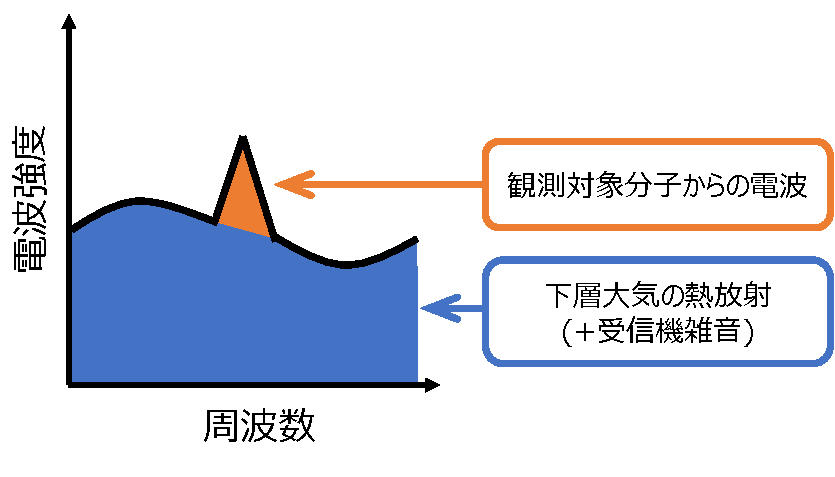
\includegraphics[width=\linewidth]{master_thesis_contents/master_thesis_fig/spectum_thermalnoise.pdf}
    \caption{スペクトルデータの強度を決める要素}
    \label{fig:spectum_thermalnoise}
\end{figure}
式\eqref{eq:absorption_selfemission_6}の左辺$T$が観測値として直接的に得られる電波強度であるが、我々が知りたい値は、もともとの放射強度である$T_0$であるので、$T_0$を知るためには光学的厚みの補正が必要となるわけである。\par

次に、光学的厚みをどのように測定するかについて述べる。
光学的厚みの測定は図\ref{fig:opticaldepth_measurement}のように観測の間に定期的に行われており、たとえばトロムソの観測装置ではおよそ5分おきに測定されている。
% 昭和基地も同じなのか?
\begin{figure}[htbp]
    \centering
    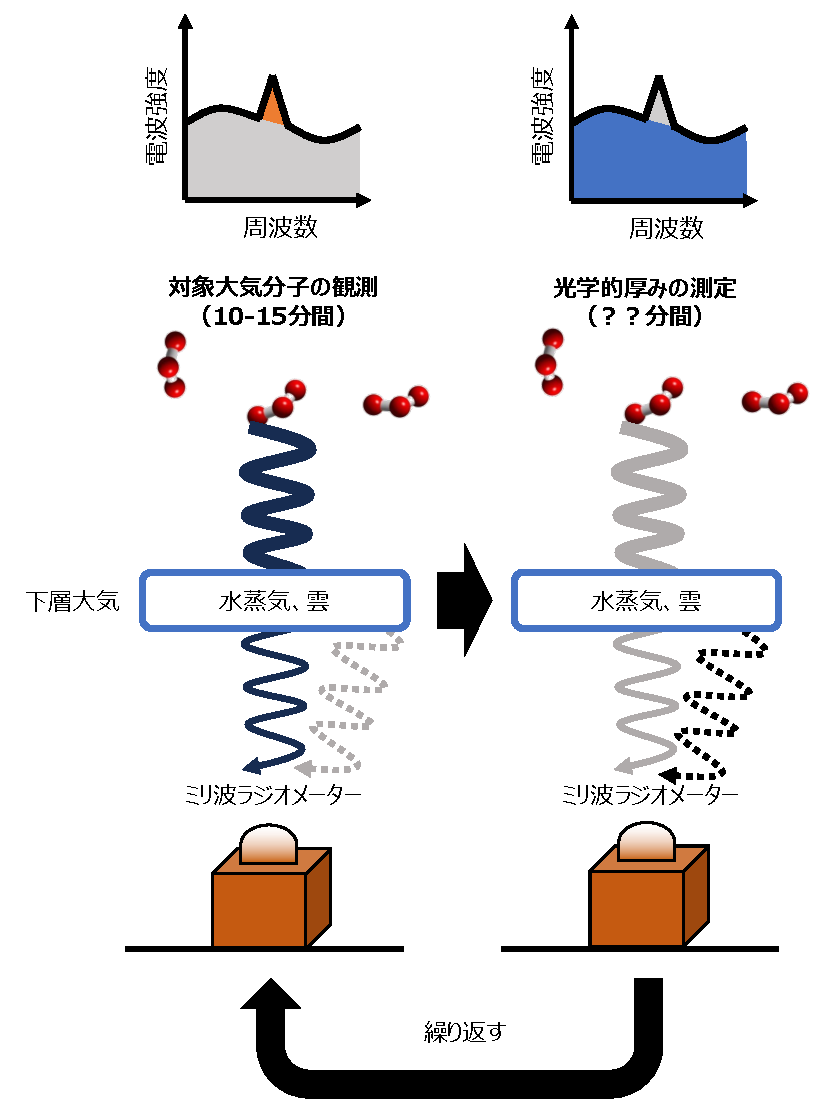
\includegraphics[width=\linewidth]{master_thesis_contents/master_thesis_fig/opticaldepth_measurement.pdf}
    \caption{ミリ波観測と光学的厚み$(\tau)$の測定の流れ}
    \label{fig:opticaldepth_measurement}
\end{figure}
% この図は必要でしょうか?図が無いと理解できないほどの内容ではないのと、図が何を説明したいのか、良く分かりませんでした。
測定された光学的厚みの値は、直前に観測された電波強度のデータの補正に用いられる。
光学的厚みの測定についてはSky tippingと呼ばれる手法が用いられる。
% Sky tippingの文献がありませんか。
まず関係式として、以下の二式を用いる。
\begin{gather}
    \begin{cases}
        T_z = T_\mathrm{sky} \left\{ 1-\exp \left(-\tau \sec z \right)  \right\} + T_\mathrm{sys} \\
        T_\mathrm{obs\_ hot} = T_\mathrm{hot} + T_\mathrm{sys}
    \end{cases}
    \label{eq:opticaldepth_measurement} \\ \notag
    z :観測する角度の天頂角 \\ \notag
    T_\mathrm{z} :天頂角zでの分子スペクトルを含まない周波数の信号強度 \\ \notag
    % T_{sky} :大気からの熱放射、T_{sys} :観測装置の自己雑音温度 \\ \notag
    T_\mathrm{obs\_ hot} :常温黒体を見たときの輝度温度 \\ \notag
\end{gather}
ここで、$T_\mathrm{sky} = T_\mathrm{hot}$と仮定し式\eqref{eq:opticaldepth_measurement}の2式の差をとって両辺対数をとると
\begin{equation}
    \ln \left( T_{obs\_ hot} - T_z \right)  = \ln T_{obs\_ hot} - \tau \sec z
    % \ln \( T_{obs\_ hot} - T_z \) = \ln T_{obs\_ hot} - \tau \sec z
\end{equation}
となる。
この式は$y=ax$のような一次関数になっているため、左辺$\ln \left( T_\mathrm{obs\_ hot} - T_z \right)$を縦軸、$\sec z$を横軸としたプロットを作成すると、図\ref{fig:opticaldepth_slope_tau}のようになることがわかる(プロットデータは観測装置の回転鏡により$z$の値を変えている)。
これらのプロットに対して一次の近似直線を引いたとき、その直線の傾きが光学的厚みに負の符号をつけたものと対応する。
以上より、光学的厚みを観測的に求めることができる。\par
\begin{figure}[htbp]
    \centering
    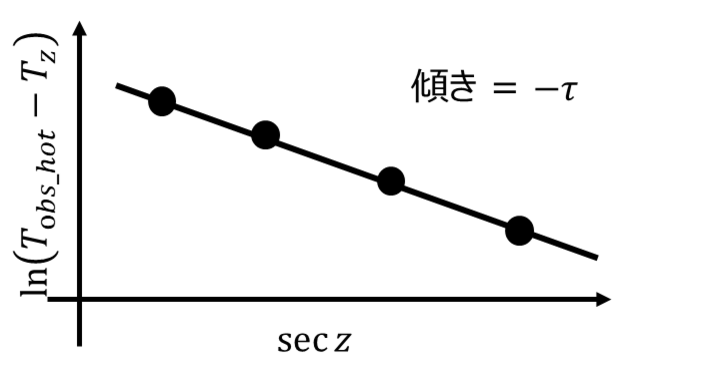
\includegraphics[width=\linewidth]{master_thesis_contents/master_thesis_fig/opticaldepth_slope_tau.pdf}
    \caption{光学的厚み$\tau$を求めるためのプロットデータの模式図}
    \label{fig:opticaldepth_slope_tau}
\end{figure}
トロムソの観測装置で実際に測定している$\sec z$の値は、表\ref{tb:secz_zdeg}のようになっている。
ここでは、それに対応した天頂角$z$と仰角の値も示す。
\begin{table}[htbp]
    \centering
    \caption{$\sec z$と天頂角$z\ [ \deg ]$と仰角$[ \deg ]$との対応}
    \label{tb:secz_zdeg}
    \setlength{\belowcaptionskip}{5mm}
    \begin{tabular}{ccc}
    \hline
    $\sec z$ & 天頂角 $z\ [ \deg ]$ & 仰角$[ \deg ]$ \\ \hline
    1.46 & 47 & 43 \\ \hline
    1.83 & 57 & 33 \\ \hline
    2.28 & 64 & 26 \\ \hline
    2.79 & 69 & 21 \\ \hline
    \end{tabular}
\end{table}


\subsection{周波数スイッチング}
\label{subsec:frsw}
観測されたスペクトルデータから対象の分子スペクトルのみを得るためには、大気の熱放射と観測装置の受信機雑音によるオフセット成分を除去する必要がある。
このオフセットを除去するにはいくつかの手法が行われているが、本研究で使用する観測装置では、周波数スイッチング(以後FRSWとする)という手法を用いる。
% (図\ref{fig:frsw_schema})
% \begin{figure}[htbp]
%     \centering
%     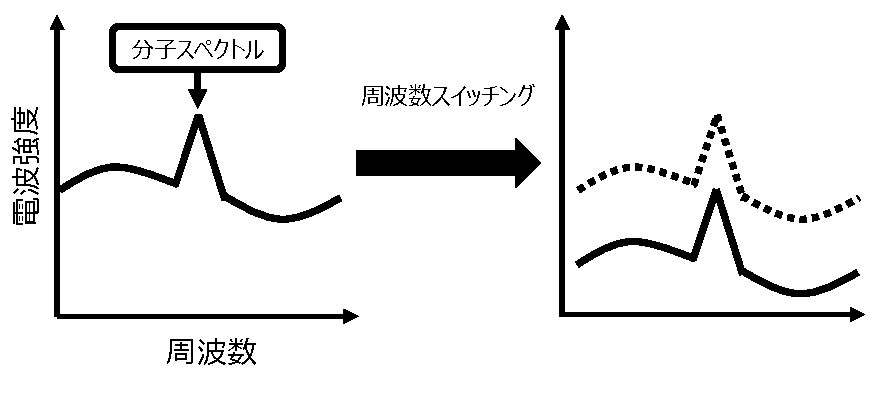
\includegraphics[width=\linewidth]{master_thesis_contents/master_thesis_fig/frsw_schema.pdf}
%     \caption{周波数スイッチング(FRSW)の模式図}
%     \label{fig:frsw_schema}
% \end{figure}
% 図は必要なしか。
ただし、FRSWによるオフセット成分の除去はおおまかなものであるため、本研究のように弱いスペクトルを検出する必要がある場合には、さらに細かくオフセット成分を補正する処理が必要となる(詳細は\ref{sec:correction_baselinefitting}節で述べる)。
本研究では、ハードウェアでのFRSWによるデータ取得に加えて、周波数折返し処理という解析方法を用いる。
この手法を用いることで、オフセット成分を除去するとともに、スペクトルデータの信号対雑音比(S/N比)を向上させている。\par

\begin{figure}[htbp]
    \centering
    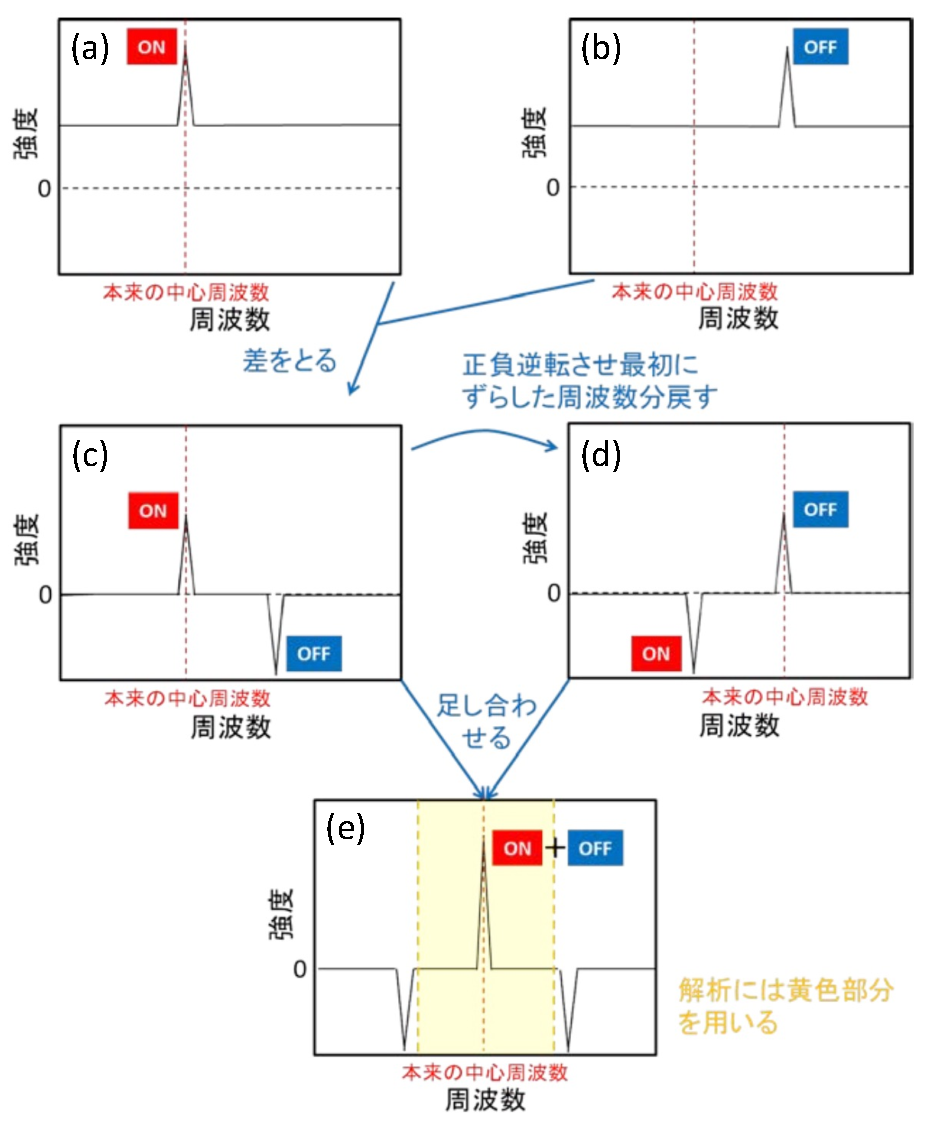
\includegraphics[width=\linewidth]{master_thesis_contents/master_thesis_fig/frsw_process.pdf}
    \caption{周波数スイッチングと周波数折り返し処理の概要(\cite{ito2017master}より引用)}
    \label{fig:frsw_process}
\end{figure}
まず、ハードウェア的に行われるFRSWについて説明する。
ある周波数において最初に取得されるデータを図\ref{fig:frsw_process}(a)に示す。
次に、局部発振器の周波数を$\Delta f$ずらした状態でデータを取得する(図\ref{fig:frsw_process}(b))。
これにより、分光計のチャンネル上では、異なるチャンネルに同じ分子からの輝線スペクトルが現れる2つのデータが得られる。
その次に、解析では、まず(a)から(b)を差し引いたデータを作成する(図\ref{fig:frsw_process}(c))。
これにより、(a)と(b)に共通に乗っていたオフセット成分が差し引かれる。
さらに(c)を上下反転して、ずらした周波数$\Delta f$を戻した(d)を作成する。
この(d)と(c)のデータを足し合わせて2で割る処理をする(周波数折り返し処理)。
(a)と(b)で取得された輝線スペクトルのデータは独立なものなので、この処理をすることによって、大気雑音や受信機雑音などのランダムなノイズ成分が低減し、S/N比としては$\sqrt{2}$倍向上する(図\ref{fig:frsw_process}(e))。
そして、最終的に得られる分子スペクトルとしては、図\ref{fig:frsw_process}(e)中の黄色で囲まれたところのみを使う。
\clearpage


\section{観測場所}
\label{sec:obs_location}
\ref{sec:obs_location}節では、解析に用いたノルウェーのトロムソと南極の昭和基地のミリ波分光計について、それぞれ観測を立ち上げた時期と設置されてきた分光計の概要を述べる。トロムソと昭和基地で設置された分光計の仕様を表\ref{tb:spectrometer_spec}に示す。
\begin{table}[htbp]
    \centering
    \caption{トロムソ(1段目)と昭和基地(2段目)で設置された分光計の仕様}
    \label{tb:spectrometer_spec}
    \setlength{\belowcaptionskip}{5mm}
    \resizebox{\columnwidth}{!}{%
    \begin{tabular}{ccccc}
    \hline
    &
        期間 &
        FrontEnd &
        BackEnd &
        観測対象の分子 \\ \hline
    単周波数分光計 &
        2016年 - &
        \begin{tabular}[c]{@{}c@{}} Double sideband\\ PCTJ  SIS mixer\end{tabular} &
        \begin{tabular}[c]{@{}c@{}}FFT 分光計\\ 帯域 $\sim1\ \mathrm{GHz}$\\ 分解能 $\sim61\ \mathrm{kHz}$\end{tabular} &
        \begin{tabular}[c]{@{}c@{}}\ce{NO}, \ce{O3} \\ (切替観測)\end{tabular} \\ \hline
    % Multi-freq. Phase 1 &
    %     \begin{tabular}[c]{@{}c@{}}2020年11月 – \\ 2021年2月\end{tabular} &
    %     \begin{tabular}[c]{@{}c@{}}2 Single sideband\\ PCTJ SIS mixers\end{tabular} &
    %     \begin{tabular}[c]{@{}c@{}}FFT 分光計\\ 帯域 $\sim$1GHz\\ 分解能 $\sim$61 kHz\end{tabular} &
    %     \begin{tabular}[c]{@{}c@{}}\ce{NO}, \ce{O3}, \ce{CO}, \ce{HO2} \\ (分子同時観測可能)\end{tabular} \\ \hline
    % Multi-freq. Phase 2 &
    %     \begin{tabular}[c]{@{}c@{}}2021年3月 –\\ 2022年1月\end{tabular} &
    %     \begin{tabular}[c]{@{}c@{}}1 Single sideband\\ PCTJ SIS mixers\end{tabular} &
    %     \begin{tabular}[c]{@{}c@{}}FFT 分光計\\ 帯域 $\sim$2 GHz\\ 分解能 $\sim$61 kHz\end{tabular} &
    %     \begin{tabular}[c]{@{}c@{}}\ce{NO}, \ce{O3}, \ce{HO2} \\ (分子同時観測可能)\\ (due to oscillator damage)\end{tabular} \\ \hline
    多周波数分光計 &
    % 多周波数分光計 Phase 3 &
        2022年7月 - &
        \begin{tabular}[c]{@{}c@{}}2 Single sideband\\ series-array SIS mixers\end{tabular} &
        \begin{tabular}[c]{@{}c@{}}FFT 分光計\\ 帯域 $\sim2.5\ \mathrm{GHz}$\\ 分解能 $\sim76\ \mathrm{kHz}$\end{tabular} &
        \begin{tabular}[c]{@{}c@{}}\ce{NO}, \ce{O3}, \ce{CO}, \ce{NO2}, \ce{HO2}\\ (同時観測)\end{tabular} \\ \hline
    \end{tabular}
    }
\end{table}


\subsection{ノルウェー・トロムソでの観測(69.35\textdegree N, 19.14\textdegree E)}
\label{subsec:mm_tromsoe}
\ref{sec:intro_privious}節で述べたように、\ce{NO}のミリ波分光観測において、南極域の夏期には光化学反応の影響による\ce{NO}の減少によって\ce{NO}の短期変動の観測が困難になっているという課題がある。
これは、季節が逆転する北極域において同様の観測を行い、両極域で\ce{NO}の同時モニタリングをすることによって解決できる可能性がある。
なぜなら、両極において日照時間の長さは真逆の関係になっており、一方の極が夏期(極域では白夜)ならもう一方の極は冬期(極夜)になるからである。
つまり、光化学反応の影響を強く受ける夏期では原因の切り分けが難しいが、同時期にもう一方の極でデータを取得して比較することで、EPPによる短期間変動を切り分けることができると考えた。\par

我々は、北極域での観測拠点としてノルウェーのトロムソにあるEISCAT(European Incoherent Scatter)レーダー観測所に、2015年から2016年にかけて新たな観測装置を設置した~\cite{ito2017master}。
トロムソは南極の昭和基地とおよそ地理緯度が同じであるため、大きなEPPが起きると同時に影響を受けると期待できる。
また観測値として既存の観測所を利用することで、観測装置の設置や運用のために新たにインフラを整備する必要がないという利点があるほか、EISCATレーダーの観測によって得られる電離圏の電子密度などのデータを用いることで、電子降り込みに関する情報と比較することができるということも重要である。
しかし、トロムソではミリ波地上観測が行われたことが無く、とくに我々にとって、はじめての観測地である。
そのため、周囲の電波環境や下層大気の状況、さらに新たに開発された観測装置の現地での特性などは明らかではなく、実際にどのような質のデータが取れるのかということの確認がまず必要であった。\par

本研究では、取得されるデータを科学的研究に最大限に活用するために、データの傾向や特徴を精査した。
そして、その傾向や特徴からデータのスクリーニング(特定の条件を設定し、全体のデータから解析に用いることができるデータのみを選別)を行った(詳細は\ref{sec:screening_opticaldepth}節と\ref{sec:screening_spectralnoise}節にて述べる)。
今回は2018年12月26日〜2019年3月10日の期間に行われたテスト観測データを用いた。
% 観測諸元をここで説明するなら、期間だけでなく、使用データの詳細な説明が必要です。別の章に書くつもりなら、観測期間もここには必要ないでしょう。


\subsection{南極・昭和基地での観測(69.00\textdegree S, 39.85\textdegree E)}
\label{subsec:mm_syowa}
南極の昭和基地では2011年に観測装置が立ち上げられ、現在まで観測が続けられている~\cite{isono2014variations,isono2014ground}。
今回は2023年3月22日〜2023年3月30日の観測データを用いた。
% 観測諸元をどこにまとめるか?
昭和基地では、設置当初から\ce{O3}と\ce{NO}を切り替えることで、両分子のモニタリング観測が行われてきた。
これらの同時観測を行うため、2020年に新たに多周波数分光計が設置され、2022年7月より定常観測を開始した~\cite{iwata2019master,kosegaki2020master}。
% 加えて、中島のマルチプレクサ論文、作間先生の超伝導フィルタ論文を引用
一度に分光できる帯域幅は、従来の分光計と比較すると、$1\, \mathrm{GHz}$から$2.5\, \mathrm{GHz}$に広がった(表\ref{tb:spectrometer_spec})。
帯域が広がったことにより、\ce{NO}・\ce{O3}・\ce{CO}・\ce{NO2}・\ce{HO2}の5分子同時観測が実現しただけでなく、とくに\ce{NO}については輝線スペクトルの本数を増やすことができた。
% NO分子輝線は、超微細構造(これも説明が必要)を持ち、複数のラインがあることを説明する必要あり。
トロムソに設置されている分光計では、超微細構造線のうち2本の輝線スペクトルのみの観測であったが、昭和基地の新たな分光計では合計6本の輝線スペクトルを観測することができるようになった。\par

昭和基地で現在同時観測されている分子スペクトルの例を図\ref{fig:NO_spectr}に示す。
黒枠が6本の\ce{NO}スペクトルを表し、そのうち赤枠で示したもののみがトロムソで観測されている2本のスペクトルである。
それぞれの輝線スペクトルの静止周波数と遷移については、表\ref{tb:no_spectr_freq}に示す。
なお、\ce{NO}スペクトルの静止周波数および線スペクトル強度係数は、NASAが提供しているJPL Catalog\footnote{\url{https://spec.jpl.nasa.gov/ftp/pub/catalog/catform.html}}より調べた。
線スペクトル強度係数は柱密度の導出に用いるパラメーターである(詳細は\ref{sec:derive_columndensity}節)。
\begin{figure}[htbp]
    \centering
    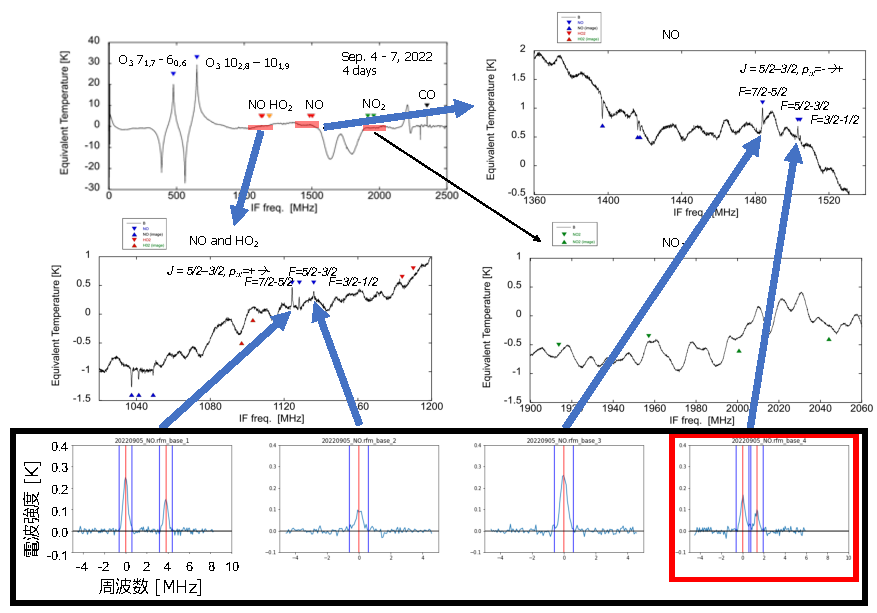
\includegraphics[width=\linewidth]{master_thesis_contents/master_thesis_fig/NO_spectr.pdf}
    % \caption{$\scriptstyle \mbox{昭和基地で現在観測できる6本の\ce{NO}輝線スペクトル} \scriptstyle
    % \mbox{(黒枠。赤枠はトロムソで観測できる2本の輝線スペクトル)}$}
    \caption{昭和基地で現在観測されている6本の\ce{NO}輝線スペクトルの例}
    % \caption{\protect 昭和基地で現在観測できる6本の\ce{NO}輝線スペクトル \linebreak
    % (黒枠。赤枠はトロムソで観測できる2本の輝線スペクトル)}
    \label{fig:NO_spectr}
\end{figure}
\begin{table}[htbp]
    \centering
    \caption{トロムソと昭和基地で観測される6本の\ce{NO}の輝線スペクトル}
    \label{tb:no_spectr_freq}
    \resizebox{\textwidth}{!}{%
    \begin{tabular}{cccccccc}
    \hline
    周波数 & \multicolumn{2}{c}{観測可能} & $J$ & $P_{\mathrm{ul}}$ & $F$ & IF 周波数  & 線スペクトル強度係数 $A$ \\
    $[\mathrm{GHz}]$ & Troms\o & Syowa &  &  &  & $[\mathrm{MHz}]$ & $[\mathrm{K^{-2}} \mathrm{MHz^{-1}} \mathrm{cm^{-2}}]$ \\ \hline
    $250.436848$ &  & $\circ$ & $5/2 - 3/2$ & \ce{+ -> -} & $7/2 - 5/2$ & $1124.3$ & $4.00\times 10^{13}$ \\ \hline
    $250.440659$ &  & $\circ$ & $5/2 - 3/2$ & \ce{+ -> -} & $5/2 - 3/2$ & $1128.2$ & $6.35\times 10^{13}$ \\ \hline
    $250.448530$ &  & $\circ$ & $5/2 - 3/2$ & \ce{+ -> -} & $3/2 - 1/2$ & $1136.0$ & $1.07\times 10^{14}$ \\ \hline
    $250.796436$ &  & $\circ$ & $5/2 - 3/2$ & \ce{- -> +} & $7/2 - 5/2$ & $1483.9$ & $3.99\times 10^{13}$ \\ \hline
    $250.815954$ & $\circ$ & $\circ$ & $5/2 - 3/2$ & \ce{- -> +} & $5/2 - 3/2$ & $1503.1$ & $6.33\times 10^{13}$ \\ \hline
    $250.816954$ & $\circ$ & $\circ$ & $5/2 - 3/2$ & \ce{- -> +} & $3/2 - 1/2$ & $1504.5$ & $1.06\times 10^{14}$ \\ \hline
    \end{tabular}%
    }
\end{table}
図\ref{fig:NO_spectr}を見ると、\ce{O3}スペクトルと比較して、\ce{NO}スペクトルはとても微弱である。
そのため、取得された全スペクトルデータのうち、どのデータが解析に用いることができるかということをあらかじめスクリーニングして抽出することが重要となる。
